\setcounter{section}{2}

\Needspace{5\baselineskip}
\hypertarget{gradient-descent-and-backpropagation}{%
\section{Gradient Descent and Backpropagation}\label{gradient-descent-and-backpropagation}}

\Needspace{5\baselineskip}
\hypertarget{i.-gradient-descent}{%
\subsection{I. Gradient Descent}\label{i.-gradient-descent}}

\Needspace{4\baselineskip}
\begin{enumerate}
\def\labelenumi{\arabic{enumi}.}
\tightlist
\item
  Basic principle
\end{enumerate}

We now have a ``machine'' (a neural network) and know how to ``score'' it (with a loss function). The next question is: how can AI ``improve itself'' based on this ``score''?

Imagine that you (the AI) are standing in an enormous n+1-dimensional mountain range (the ``surface of the loss as a function of n-dimensional parameters''), covered in dense fog (the global function cannot be solved directly). Your goal is to find the lowest ``valley'' (the minimum Loss). You cannot see where the valley floor is and can only move in the direction of ``steepest descent.''

Mathematically, the gradient is a vector whose entries are the partial derivatives of the dependent variable (Loss) with respect to each independent variable. A partial derivative can be understood as the derivative with respect to that variable while the others are held fixed: the limit of the change in the dependent variable divided by the change in that independent variable.

\[
\nabla L = \left(\frac{\partial L}{\partial \theta_1}, \frac{\partial L}{\partial \theta_2}, \ldots, \frac{\partial L}{\partial \theta_n}\right)
\]

The gradient indicates the increase in the loss as the parameters change. Since we want the loss to decrease, we place a minus sign before the gradient vector to take the opposite direction. For a model with n parameters, the negative gradient vector is an ``instruction package'' that combines the ``steepness in n directions.'' Its first entry, for example, represents ``how quickly the altitude (L) decreases when only θ1 changes.''

\begin{figure}[htbp]
\centering
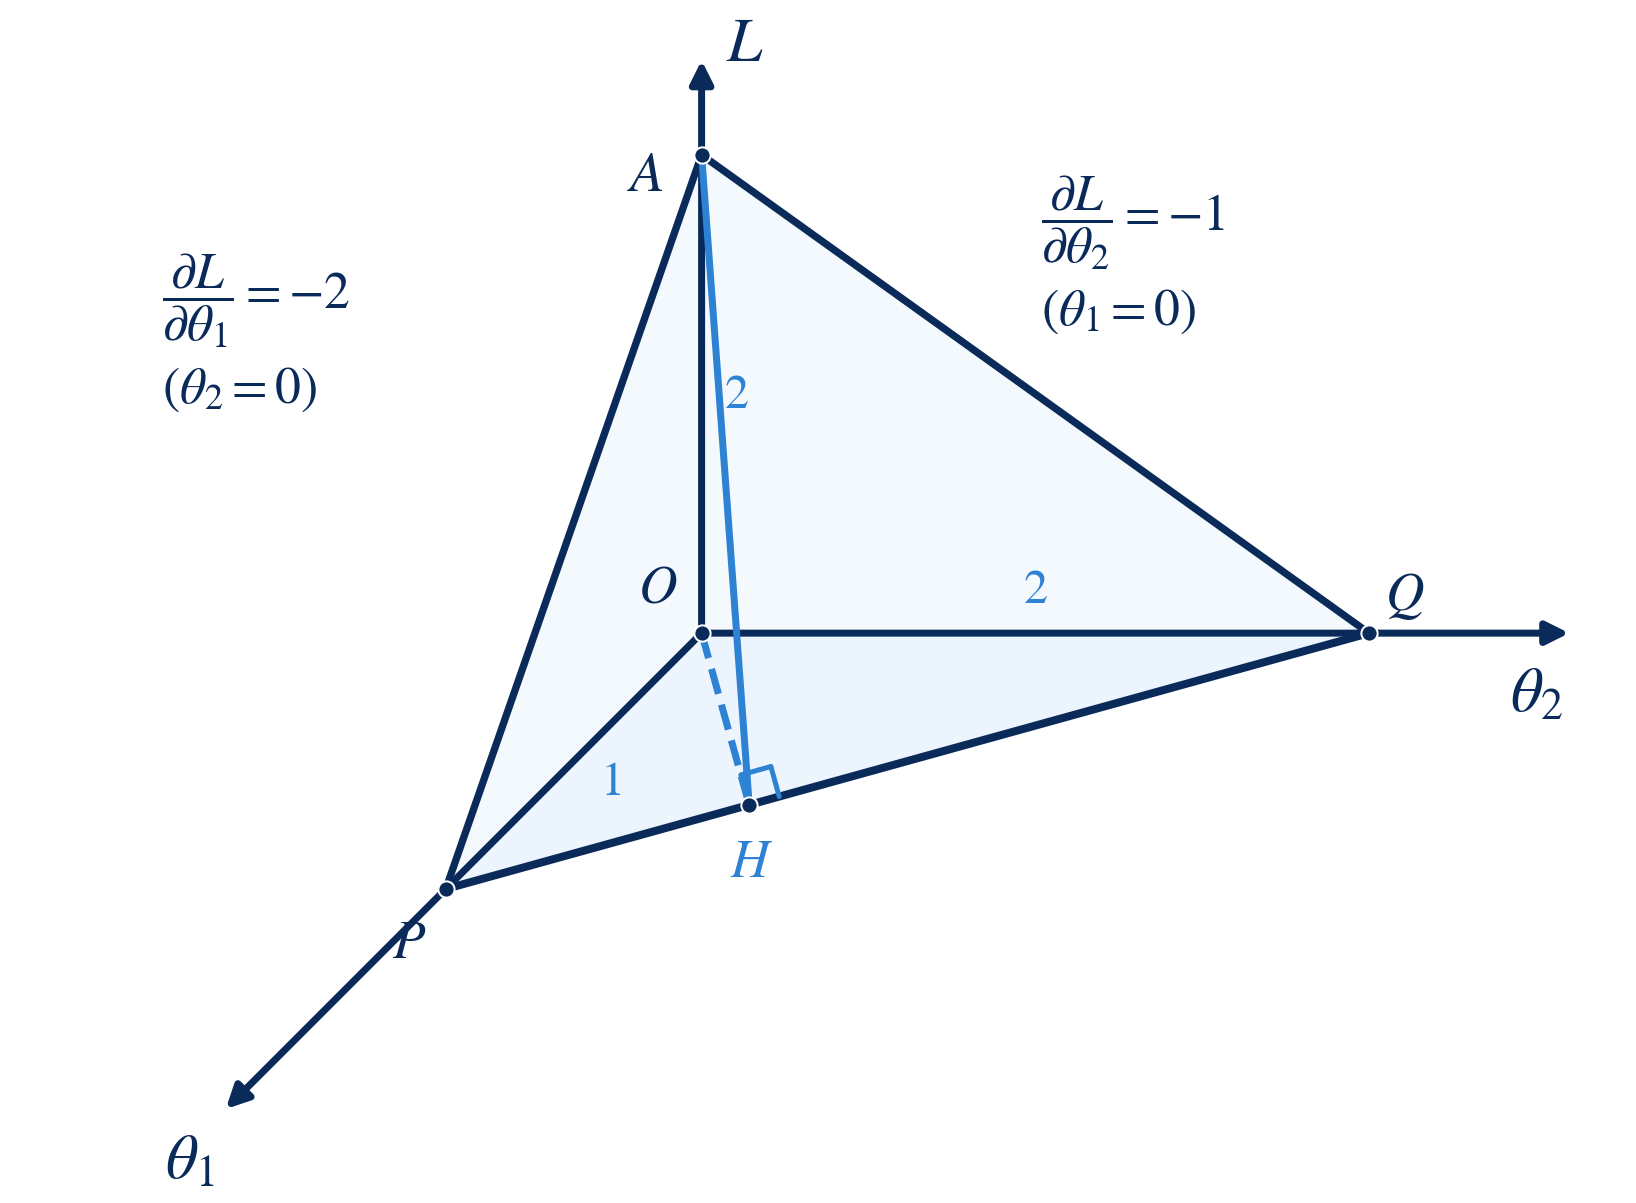
\includegraphics{images/image-0005.png}
\caption{Geometric relationship between local slopes in two parameter directions and the negative gradient}
\end{figure}

For example, the figure above has only two parameters, and the loss \(L\) is a function of \(\theta_1\) and \(\theta_2\). Point \(O\) is the intersection of the two coordinate axes in the parameter plane. Point \(A\) represents the loss when the parameters are at \(O\); \(AO\) is perpendicular to the parameter plane, and the figure sets \(AO=2\). The local tangent plane to the loss surface at \(A\) intersects the \(\theta_1\) and \(\theta_2\) axes at \(P\) and \(Q\), respectively, with \(OP=1\) and \(OQ=2\). Thus, this local tangent plane can be written as

\[
L=2-2\theta_1-\theta_2,
\qquad
\nabla L=(-2,-1),
\qquad
-\nabla L=(2,1).
\]

With \(\theta_2=0\) fixed, increasing \(\theta_1\) by 1 decreases \(L\) by 2, so \(\frac{\partial L}{\partial\theta_1}=-2\). With \(\theta_1=0\) fixed, increasing \(\theta_2\) by 2 decreases \(L\) by 2, so \(\frac{\partial L}{\partial\theta_2}=-1\). The partial derivative in the \(\theta_1\) direction therefore has the larger absolute value, and descent in that direction is steeper.

Points \(P\), \(H\), and \(Q\) lie on the same line. \(H\) is the foot of the perpendicular from \(O\) to line \(PQ\), so \(OH\perp PQ\). The projection of \(AH\) onto the parameter plane is \(OH\). Furthermore, line \(PQ\) has equation \(2\theta_1+\theta_2=2\) and normal vector \((2,1)\), so \(OH\) points in the same direction as the negative gradient \(-\nabla L=(2,1)\). This explains why the parameters should be updated in the negative gradient direction.

\Needspace{4\baselineskip}
\begin{enumerate}
\def\labelenumi{\arabic{enumi}.}
\setcounter{enumi}{1}
\tightlist
\item
  Adjusting the learning rate
\end{enumerate}

We know the direction in which to change the parameters, but how much should we change them?

Usually, we multiply the negative gradient vector by a constant called the learning rate. The learning rate is a hyperparameter; it cannot itself be optimized through gradient descent and must be adjusted manually. The two diagrams below, viewed along the L axis, show the problems that arise during parameter updates when the learning rate is too large or too small. If it is too large, ``oscillation'' may prevent the parameters from ever reaching the lowest point, or the updates may even be counterproductive. If it is too small, the step size is too small, so gradient descent requires more steps and incurs greater computation and computational overhead.

\begin{figure}[htbp]
\centering
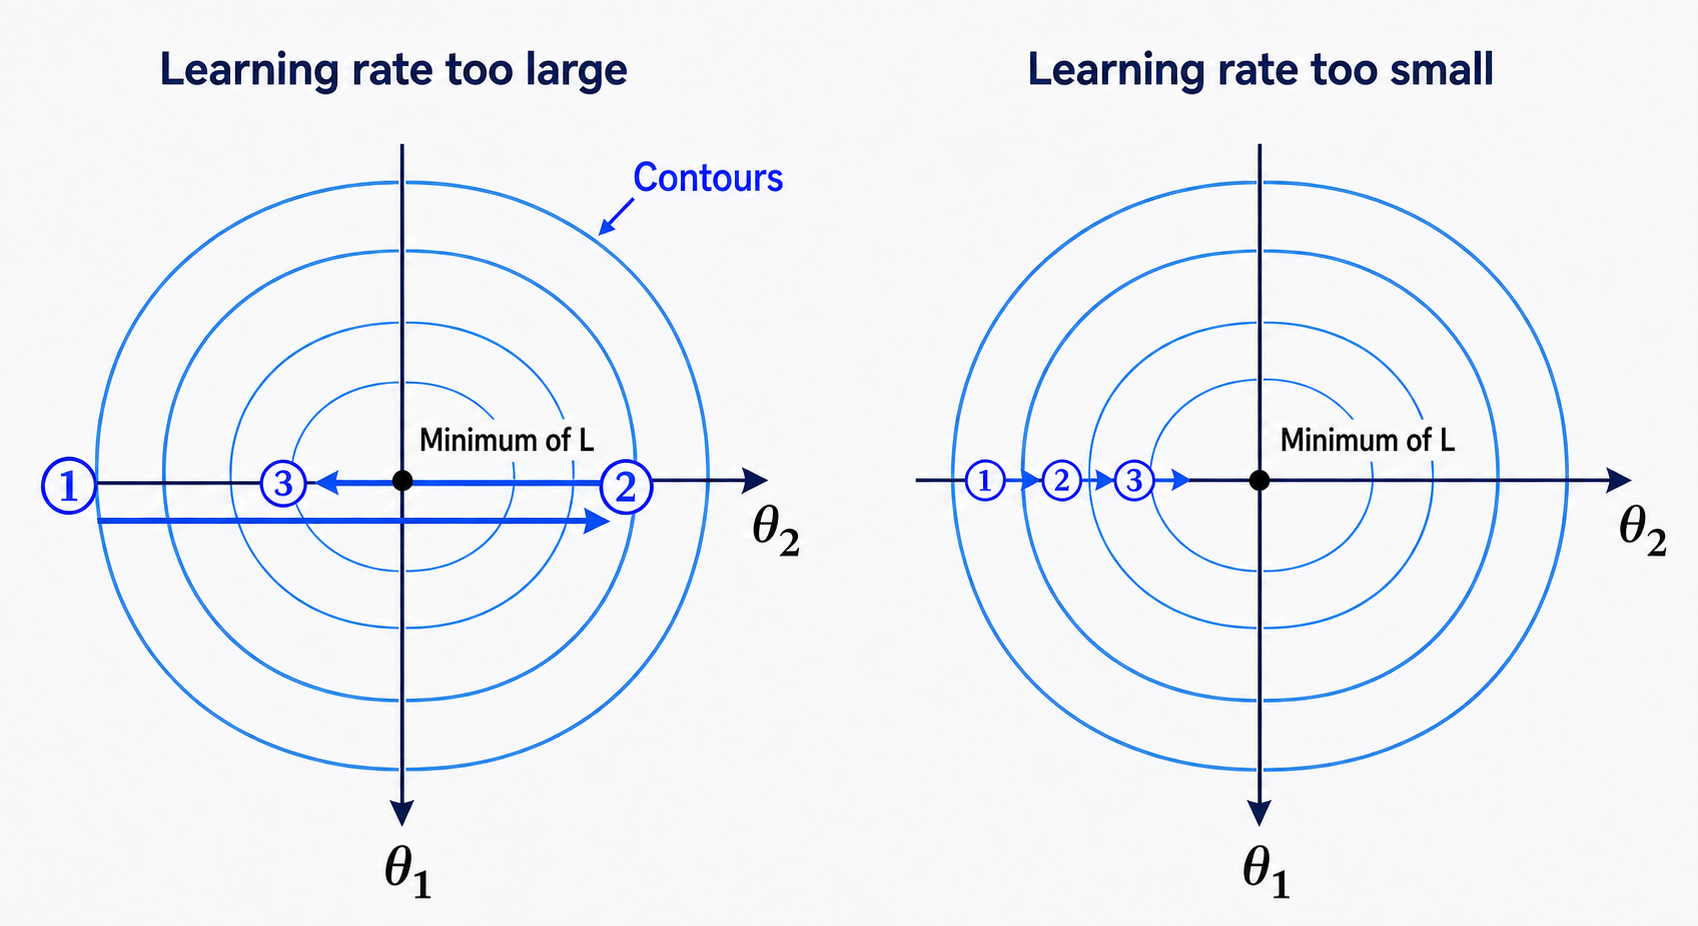
\includegraphics{images/image-0065.png}
\caption{Effects of an excessively large or small learning rate}
\end{figure}

\Needspace{4\baselineskip}
\begin{enumerate}
\def\labelenumi{\arabic{enumi}.}
\setcounter{enumi}{2}
\tightlist
\item
  Mini-batch stochastic gradient descent
\end{enumerate}

We understand gradient descent, but whose loss should Loss represent?

Taking the average over all samples is computationally expensive. Moreover, every step uses the same samples' Loss as a function of the parameters, so it lacks randomness and can easily become ``trapped'' in a local minimum without being able to ``escape.'' Using just one sample introduces too much randomness. We therefore generally divide the samples randomly into multiple mini-batches. At each step, one batch is used to compute the negative gradient of Loss with respect to the parameters and perform gradient descent, balancing accuracy, an appropriate degree of randomness, and computational overhead.

\Needspace{5\baselineskip}
\hypertarget{ii.-backpropagation}{%
\subsection{II. Backpropagation}\label{ii.-backpropagation}}

We know that AI needs to follow the negative-gradient ``instruction package'' downhill. But a crucial question remains: in a complex neural network with millions or even billions of parameters, how can we efficiently compute this ``instruction package'' containing the gradients of the loss function with respect to every parameter (the ``steepness'' in every direction)?

Backpropagation is an algorithm that uses the chain rule to compute the partial derivatives of the loss function with respect to every parameter in the network, working backward layer by layer from the output layer. We can think of it as an intricate system for allocating responsibility and error.

\Needspace{4\baselineskip}
\begin{enumerate}
\def\labelenumi{\arabic{enumi}.}
\tightlist
\item
  An intuitive analogy: a production line and tracing responsibility
\end{enumerate}

Imagine a chocolate factory (the neural network): raw materials such as cocoa powder, sugar, and milk (the input data) pass through multiple processing stages such as mixing, heating, stirring, cooling, and shaping (the network layers), producing a finished chocolate bar (the prediction). A quality inspector tastes it and provides a score, such as ``too bitter'' (computing the loss). The chocolate is now found to be too bitter (the loss is large), so the factory needs to improve. Backpropagation addresses the question: how can we determine precisely how much ``responsibility'' each stage should bear? Did the stirring stage (an intermediate layer) fail to mix thoroughly? Was the temperature wrong at the heating stage (another layer)? Or was the concentration of the purchased cocoa powder (the input data) simply too high to begin with?

\Needspace{5\baselineskip}
It traces responsibility precisely:

The quality inspector (the loss function) first determines how ``bitter'' the final product is (the gradient of loss L with respect to the output), and sends feedback to the final shaping stage: ``Your product is too bitter; the deviation is xxx.'' After receiving this feedback, the shaping stage thinks: ``I only shape the product. The bitterness mainly comes from the semifinished product sent by the cooling stage, and according to my process (activation function), this is how sensitive I am to bitterness\ldots{}'' It then combines this information with its own ``process characteristics'' (the local gradient), computes the responsibility attributed to the preceding stage (cooling), and passes that attribution backward. This process continues backward layer by layer. Each layer uses the ``attribution'' received from the following layer and its own ``process manual'' (the local function and its derivative) to determine its responsibility for the problem, then traces it further toward the earlier stages. Eventually, this error signal reaches the initial raw-material procurement (the input layer) and every individual stage. Each link in the chain then knows: ``I need to bear XX\% of the responsibility for this `bitter' result.''

\Needspace{4\baselineskip}
\begin{enumerate}
\def\labelenumi{\arabic{enumi}.}
\setcounter{enumi}{1}
\tightlist
\item
  Mathematical expression
\end{enumerate}

Mathematically, this ``tracing of responsibility'' is implemented by the chain rule in calculus, which computes derivatives of composite functions.

Consider a simple network: input layer x -\textgreater{} intermediate layer h = f(w1\emph{x) -\textgreater{} output layer y = g(w2}h) -\textgreater{} loss L(y).

\Needspace{5\baselineskip}
We want the gradient of loss L with respect to the first parameter w1. By the chain rule:

\[
\frac{\partial L}{\partial w_1}=\frac{\partial L}{\partial y}\cdot\frac{\partial y}{\partial h}\cdot\frac{\partial h}{\partial w_1}
\]

\Needspace{5\baselineskip}
Backpropagation computes the expression above from right to left:

\begin{enumerate}
\def\labelenumi{\arabic{enumi}.}
\tightlist
\item
  Forward propagation: first perform a complete computation from x to L, recording the intermediate results of each layer (h and y).
\item
\Needspace{5\baselineskip}
  Backward computation:

  \begin{enumerate}
  \def\labelenumii{\alph{enumii}.}
  \tightlist
  \item
    First compute \(\frac{\partial L}{\partial y}\) (the gradient of the loss with respect to the output).
  \item
    Then multiply this gradient by \(\frac{\partial y}{\partial h}\) (the gradient of the output with respect to the intermediate layer) to obtain \(\frac{\partial L}{\partial h}\) (the gradient of the loss with respect to the intermediate layer). This propagates the error from output layer y to intermediate layer h.
  \item
    Next, multiply \(\frac{\partial L}{\partial h}\) by \(\frac{\partial h}{\partial w_1}\) (the gradient of the intermediate layer with respect to parameter w1) to obtain the desired \(\frac{\partial L}{\partial w_1}\).
    Similarly, the gradient of L with respect to w2 is the gradient of L with respect to y multiplied by the gradient of y with respect to w2. Once the gradients of L with respect to all layers have been computed, gradient descent can be performed.
  \end{enumerate}
\end{enumerate}

\Needspace{5\baselineskip}
\hypertarget{iii.-vanishing-and-exploding-gradients}{%
\subsection{III. Vanishing and Exploding Gradients}\label{iii.-vanishing-and-exploding-gradients}}

\Needspace{5\baselineskip}
\hypertarget{causes}{%
\subsubsection{(1) Causes}\label{causes}}

During backpropagation, computing the gradients of parameters close to the input layer requires multiplying together the gradients of all subsequent layers. For an L-layer network, the gradient of the loss with respect to the first-layer weights \(W^{[1]}\) is:

\[
\begin{aligned}
\frac{\partial L}{\partial W^{[1]}}
&=
\frac{\partial L}{\partial a^{[L]}}
\cdot
\frac{\partial a^{[L]}}{\partial z^{[L]}}
\cdot
\frac{\partial z^{[L]}}{\partial a^{[L-1]}} \\
&\quad \cdots
\cdot
\frac{\partial a^{[2]}}{\partial z^{[2]}}
\cdot
\frac{\partial z^{[2]}}{\partial a^{[1]}}
\cdot
\frac{\partial a^{[1]}}{\partial z^{[1]}}
\cdot
\frac{\partial z^{[1]}}{\partial W^{[1]}} .
\end{aligned}
\]

In a deep network, if most of these terms have absolute values less than 1, their product approaches 0 exponentially. Parameter updates become extremely small, and the early layers almost stop learning, with negligible parameter changes. The deep network degenerates into a shallow network in which only the last few layers learn, preventing it from exploiting the representational power of a deep model. Training becomes extremely slow or even stops entirely.

Conversely, if most terms have absolute values greater than 1, the result grows exponentially toward infinity, making the weight updates extremely large. Parameter-update steps become huge and unstable, causing the loss function to oscillate sharply and fail to converge. Model parameters may become NaN (not a number) because the updated values exceed the computer's floating-point representation range. The model becomes completely unable to learn meaningful patterns.

\Needspace{5\baselineskip}
\hypertarget{solutions}{%
\subsubsection{(2) Solutions}\label{solutions}}

\begin{enumerate}
\def\labelenumi{\arabic{enumi}.}
\item
  Choice of activation function: use ReLU, whose derivative is always 1 when x \textgreater{} 0, rather than Sigmoid, whose derivative approaches 0 when x is very large or very small.
\item
  Parameter initialization techniques: these will be introduced later.
\item
  Batch normalization: force each layer's inputs back to a standard normal distribution so that the overall gradient of that layer is as close to 1 as possible.
\item
  Model architecture design: ResNet, for example, uses ``output=x+f(x)'' (where x is the input and f is a model layer) to create a ``gradient highway'' directly from input x to the output. Gradients can flow directly to shallower layers without loss, fundamentally resolving vanishing gradients in deep networks (such as ResNets with hundreds of layers).
\item
  Gradient clipping: to address exploding gradients, check the gradient norm (the length of the gradient vector) before updating the weights. If it exceeds a specified threshold, scale the gradient proportionally in every direction so that its norm (length) is within the threshold:
\end{enumerate}

\Needspace{5\baselineskip}
If \(\lVert g\rVert > \text{threshold}\), then:

\[
g\leftarrow \frac{\text{threshold}}{\lVert g\rVert}\cdot g
\]

\FloatBarrier
\Needspace{5\baselineskip}
\hypertarget{references-2}{%
\subsection{References}\label{references-2}}

\vspace{0.25em}
\begin{itemize}
\tightlist
\item
  Rumelhart, D. E., Hinton, G. E., \& Williams, R. J. (1986). \href{https://doi.org/10.1038/323533a0}{Learning representations by back-propagating errors}. Nature.
\end{itemize}

\clearpage
